\documentclass[12pt]{article}
\usepackage[english]{babel}
\usepackage[utf8x]{inputenc}
\usepackage[T1]{fontenc}
\usepackage{scribe}
\usepackage{listings}
\usepackage{graphicx}
\usepackage{tikz}
\usepackage{amsmath}
\usepackage{algpseudocode}
\usepackage{textgreek}
\def\Hat{\mkern-3mu\text{\textasciicircum}}

 
\graphicspath{{./images/}}


\Scribe{Group 22}
\Lecturer{Abir De}
\LectureNumber{20}
\LectureDate{5 April 2023}
\LectureTitle{Introduction to Deep Learning}

\lstset{style=mystyle}

\begin{document}
	\MakeScribeTop

%#############################################################
%#############################################################
%#############################################################
%#############################################################

\section{Introduction}

\subsection{Capacity of the perceptron}
What kind of function can a neural network represent ? \\
Let’s start with the simplest neural network, the Perceptron. It is effectively a NN with a single hidden layer having 1 hidden unit with an activation function σ. Both the input layer and the weights are a 1 × n vector.

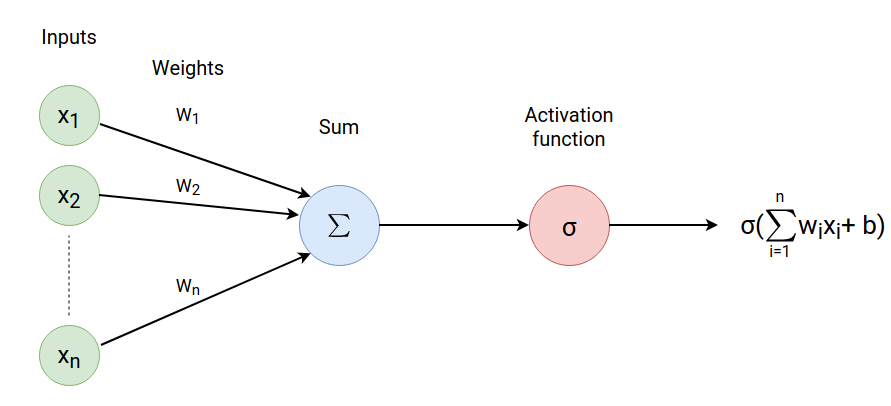
\includegraphics[width=\textwidth]{figures/perceptron.png}

The perceptron can model a function of this form: $\sigma(\sum_i^{n} \mathbf{w_i} x_i +b) = \sigma(\mathbf{w}^\top \textbf{x} + b)$. Often, we select the non-linear function $\sigma$ to be one of the following:

\begin{subequations*}
  \begin{tabularx}{\textwidth}{}
  \begin{equation*}
     \text{sigmoid} = \frac{1}{1+e^{-x}}
  \end{equation*}
  & &
  \begin{equation*}
     \text{tanh} = \frac{e^{2x}-1}{e^{2x}+1}
  \end{equation*}
    & &
  \begin{equation*}
     \text{ReLU} = \text{max}(0, x)
  \end{equation*}
  \end{tabularx}
\end{subequations*}

Notably, the Perceptron is a linear classifier, and as such it famously can’t model an XOR. \\
{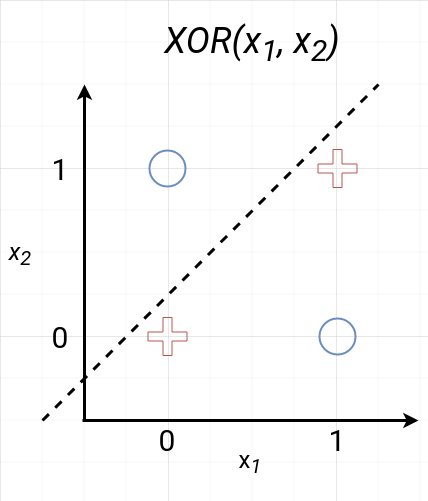
\includegraphics[height = 8cm]{figures/xor_non_linsep.png}}


\subsection{Capacity of multiple neurons}
By allowing ourselves more than 1 neuron in the hidden layer, we can model a XOR and in fact, we get the simplest \textbf{universal approximator}. \\

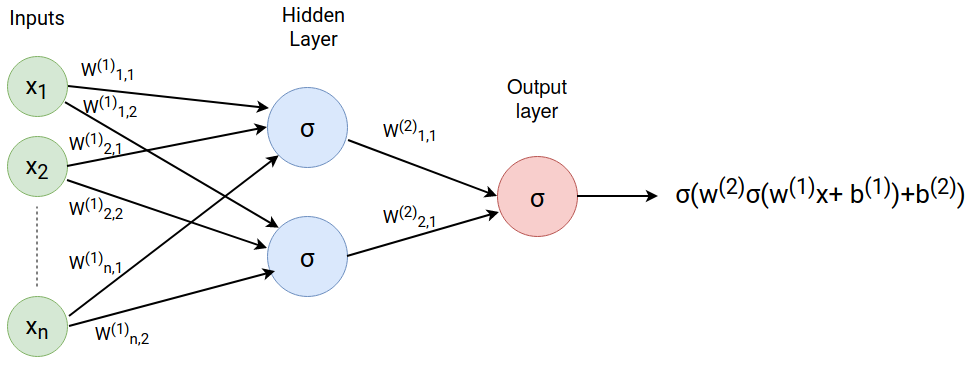
\includegraphics[width=\textwidth]{figures/nn.png}

\section{Universal Approximation theory}

The universal approximation theorem states that any continuous function $f :[0,1]^n \xrightarrow{} [0,1]$ can be approximated arbitrarily well by a neural network with at least 1 hidden layer with a finite number of weights.


\section{Deep Learning}

\subsection{Goal}
We are trying to model:
\begin{gather*}
        y = w^T \phi (x) \\
\text{but } \phi \text{ can be any non linearity. So how to model it to cover all types of functions?}
\end{gather*}
Take a linear function:
 f(x) = A\textsuperscript{m x d} x \\ \\
 Now let's apply a non-linear function g such as relu, sigmoid or tanh to all the points and get a vector. We get: \\ \\
\begin{gather*}
g(Ax) = Relu(Ax)\ or\ tanh(Ax)\ or\ \sigma (Ax)
\end{gather*}
Next, let's apply another linear function h. This can be achieved by multiplying it by a matrix B. So we get:
\begin{gather*}
h(g(Ax) = B g( Ax )
\end{gather*}
As per the universal approximation theorem, If non linear function is fixed, then there exists an A and B which can model any arbitrary non linear function.\\
'm' will determine how close it is to the original function.
\begin{gather*}
    \lVert B g(Ax) - w^T \phi(x) \rVert < \epsilon
\end{gather*}
\subsection{Algorithm}
Our goal is to minimize the following loss function:
\begin{gather*}
    \min_{A,B} \sum (y_i - Bg(Ax))^2\\
\text{So we start with random A and B and perform gradient descent:}\\
A_{t+1} \leftarrow A_t - r \Delta_A \ l(A,B) \rvert_{A_t,B_t} \\
B_{t+1} \leftarrow B_t - r \Delta_B \ l(A,B) \rvert_{A_t,B_t}
\end{gather*}
To deal with multiple minimas and to find the global minima, we repeat the process with another set of A and B multiple times. in the end, we compare losses from all sets and choose the minimum one.
\begin{samepage}
\begin{algorithmic}
\For{$t \in 1$ \ldots $T$}
\State $loss \gets 0$
\For {$i \in D$}
\State $loss += (y_i - Bg(Ax))^2$
\State $L \gets loss$
\State $A,B \gets Gradient Descent (L)$
\EndFor
\EndFor
\end{algorithmic}
\end{samepage}
However, we run into a problem here. Since we are using for loop, it will take a tremendous amount of time to calculate the loss. Because we are calculating loss for individual points.
This can be avoided if we tensorize the loss. and calculate the loss matrix and sum it as follows:
\begin{gather*}
    L = (Y - Bg(AX))^2 \\
    L = L.sum()
\end{gather*}
However we run into another problem as this we require a lot of memory. So to rectify this we tensorize in parts. This process is called batching and it allows for best utilization of memory
\subsection{Batching}

\subsubsection{How to modify the algorithm}

Divide the dataset into random batches. For doing so, we can use numpy function \lstinline{numpy.random.shuffle()}. Dimension of X is taken as N x d, batch size = b. So the modified code would look like
\begin{algorithmic}
\For{$t \in 1$ to $T$}
\State $loss \gets 0$
\State $Index \gets $ Permute(1..dim(Y))
\State $X^{'} \gets $ X[Index]
\For {$i \in 0$ to $\lfloor N/b\rfloor - 1$}
\State $X^{"} \gets $ $X^{'}$[ib:(i+1)b]
\State $Y^{"} \gets $ $Y^{'}$[ib:(i+1)b]
\State $L \gets $ $(Y^{"} - B(g(AX^{"})))^{2}$.sum()
\State $A,B \gets$ gradDes(L)
\EndFor
\EndFor
\end{algorithmic}
% describe the code here 
But why we are randomly splitting the dataset to take one batch from it?\\ 
If we perform gradient descent on entire dataset it will be slow. Instead we are permuting the dataset, taking a batch from it and performing gradient descent on that batch. It is faster. To do so, we need to keep in mind that the batch that we are selecting should represent the entire dataset. If we choose a batch without permuting the data, it might overfit one particular batch. On the other hand, if we are performing gradient descent on the entire dataset it might underfit.

% \subsection{Increasing Efficiency}
% We can use a few techniques to increase the efficiency of our algorithm. Some of them are given below.
% \subsubsection{Batch Normalization}
% \begin{algorithmic}
%     \State $X^{"} \gets \frac{X^{"} - X^{"}.mean()}{X^{"}.std()}$
% \end{algorithmic}
% \subsubsection{Dropout}
% By using dropout we will be reducing the size of the batch by some percentage at every step, lets say 70\%. So at every step we are reducing 70\% of data. As the reduction is random there won't be much loss. And this technique also reduces the possibility of overfittin\\

\section{References}
[1] http://mitliagkas.github.io/ift6085-2020/ift-6085-lecture-10-notes.pdf



%%%%%%%%%%% If you don't have citations then comment the lines below:
%
% \bibliographystyle{abbrv}           % if you need a bibliography
% \bibliography{mybib}                % assuming yours is named mybib.bib


%%%%%%%%%%% end of doc
\end{document}
